\subsubsection{EEE571 Extra Credit Problem: SymPy Solution for Circuit Analysis}

This JupyterLab notebook provides a step-by-step symbolic solution using SymPy for the 3-phase parallel RLC circuit in the Extra Credit Problem. The circuit is a three - phase circuit and has per phase:

AC source:
\begin{equation}
10\sqrt{3}\; \left[kV\right]\; Line\;to\;Line \;RMS
\end{equation}
\begin{equation}
\omega=377 \left[\frac{rad}{s}\right]
\end{equation}

The source is connected with parallel comnination of R ($1\; \Omega$), L ($j1\; \Omega$ reactance), C (100 MVA total rating). \newline

We have the following circuit conditions:
Pre-switching: steady-state.  For this state, we will compute the initial conditions using phasor analysis.

Post-switching (S opens at $i_{total} = 0$): For the state when the switch opens at the source current equal to 0A, we have free parallel RLC oscillations.

We will plot $v_C(t)$ and $i_L(t)$ to visualize each waveform.

\subparagraph{Imports and Setup}

\begin{verbatim}
import sympy as sp
import numpy as np
import matplotlib.pyplot as plt
from sympy import I, Abs, sqrt, exp, cos, sin, symbols, re, pi, arg
sp.init_printing(use_unicode=True)
\end{verbatim}

\paragraph{Analysis Steps}

\subparagraph{Step 1: Derive Circuit Parameters}

In this step, we symbolically define the given parameters and derive the per-phase capacitance $C$, inductance $L$, and capacitive reactance $X_C$. The source is line-to-line RMS voltage $V_{LL,rms} = 10\sqrt{3}$ kV at $\omega = 377$ rad/s. Capacitor rating is 100 MVA (3-phase), inductor $j1 \Omega$, resistor $R=1 \Omega$.

Per phase: $V_{ph\_rms} = V_{LL\_rms}/\sqrt{3}$, $Q_{C\_ph} = 100/3$ MVA, $X_C = V_{ph\_rms}^2 / Q_{C\_ph}$, $L = 1/\omega$, $C = 1/(\omega X_C)$.

\begin{verbatim}
omega = symbols(r'\omega', real=True, positive=True)
R = symbols('R', real=True, positive=True)

XL = symbols('X_L', real=True, positive=True)
XC = symbols('X_C', real=True, positive=True)

V_llrms = symbols('V_llrms', real=True, positive=True)
Q_c3ph = symbols('Q_c3ph', real=True, positive=True)

L = XL / omega
C = 1 / (omega * XC)
\end{verbatim}

\subparagraph{RMS Phase Voltage}

\begin{verbatim}
V_ph_rms = V_llrms / sp.sqrt(3)
V_ph_rms
\end{verbatim}

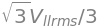
\includegraphics[width=0.7\linewidth]{files/ca092744098412576e7ecd67f2917045.png}

\subparagraph{Per Phase Capacitor Reactive Power Capacity}

\begin{verbatim}
Q_cph = Q_c3ph / 3
Q_cph
\end{verbatim}


\includegraphics[width=0.7\linewidth]{files/04c46c797cefe0314ea1594b2530d51f.png}

\subparagraph{Capacitive Reactance Equation}

\begin{verbatim}
Xc_eq = (V_ph_rms)**2 / Q_cph
Xc_eq
\end{verbatim}


\includegraphics[width=0.7\linewidth]{files/8e18de6975feda57ddc84105df2d6ab8.png}

\subparagraph{Inductance Equation}

\begin{verbatim}
L_eq = XL / omega
L_eq
\end{verbatim}


\includegraphics[width=0.7\linewidth]{files/5f0134b110d3087f888e0e734bbe04db.png}

\subparagraph{Capacitance Equation}

\begin{verbatim}
C_eq = 1 / (omega * Xc_eq)
C_eq
\end{verbatim}

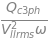
\includegraphics[width=0.7\linewidth]{files/82a5ac6bec7a430fd81ed9bc943899ab.png}

\subparagraph{Substitute Values to Calculate Capacitive Reactance}

\begin{verbatim}
numerical_subs = {omega: 377, R: 1, XL: 1, V_llrms: 10e3*sp.sqrt(3), Q_c3ph: 100*10**6}
numerical_subs
\end{verbatim}


\includegraphics[width=0.7\linewidth]{files/acfd66337a69665499ce50d439c15e78.png}

\begin{verbatim}
calc_Xc = Xc_eq.subs(numerical_subs).doit().evalf()
calc_Xc
\end{verbatim}


\includegraphics[width=0.7\linewidth]{files/a1c593464ece0d5abd9ea507659f38b4.png}

\subparagraph{Display Results of Calculating Inductance, Capacitance and Capacitive Reactance}

\begin{verbatim}
display(sp.Eq(sp.symbols('C'), C_eq))  # Symbolic expression
C_num = C_eq.subs(numerical_subs).doit().evalf()
print(f"Numerical C = {C_num:.2e} F ({C_num*1e6:.0f} \muF)")
L_num = L_eq.subs(numerical_subs).doit().evalf()
print(f"Numerical L = {L_num:.2e} H")
Xc_num = Xc_eq.subs(numerical_subs).doit().evalf()
print(f"Numerical X_C = {Xc_num:.2f} \Omega")
\end{verbatim}

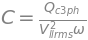
\includegraphics[width=0.7\linewidth]{files/cce0708ffbdf7d8ee103fe83fbac39ec.png}

\begin{verbatim}
Numerical C = 8.84e -4 F (884 \muF)
Numerical L = 2.65e -3 H
Numerical X_C = 3.00 \Omega
\end{verbatim}

\textbf{Output (Symbolic):}

\begin{equation}
C = \frac{Q_{c3ph}}{V_{llrms}^{2} \omega}
\end{equation}

\textbf{Numerical Values:}\newline
\begin{equation}
C \approx 8.84 \times 10^{-4}\; \left[F\right]\; \left(884\;μF\right)
\end{equation}
\begin{equation}
L \approx 2.65 \times 10^{-3}\;\left[H \right]
\end{equation}
\begin{equation}
X_C = 3 \; \left[Ω\right]
\end{equation}
\begin{equation}
V_{ph\_rms} = 10000 \left[V\right]
\end{equation}

\subparagraph{Step 2: Steady-State Analysis (Pre-Switching Phasors)}

Steady-state ($t<0$):

Admittances:
\begin{equation}
Y_R=1/R
\end{equation}

\begin{equation}
Y_L=1/(j X_L)
\end{equation}

\begin{equation}
Y_C=j/ X_C
\end{equation}

\begin{equation}
Y_{total} = Y_R + Y_L + Y_C
\end{equation}

\begin{equation}
I_{total\_rms} = V_{ph\_rms} \times Y_{total} \left(V_ph ∠0° initial\right)
\end{equation}

Switch at $i_{total}=0$:

Adjust $V_{ph}$ phase:

\begin{equation}
\theta = \frac{\pi}{2} - \angle{Y_{total}}
\end{equation}

Therefore:
\begin{equation}
\angle{I_{total}} = \frac{\pi}{2}
\end{equation}

\begin{equation}
i\left(t\right)=I_{peak} cos\left(\omega t + \frac{\pi}{2}\right) = -I_{peak} sin\left(\omega t\right), zero\;at\;t=0)
\end{equation}

and:

\begin{equation}
v\left(0\right) = \sqrt{2} Re\left[V_{ph\_rms} e^{jθ}\right]
\end{equation}

\begin{equation}
i_{L}\left(0\right) = \sqrt{2} Re\left[\frac{V_{ph\_rms} e^{jθ}}{j X_L}\right].
\end{equation}

\subparagraph{Inductive Impedance}

\begin{verbatim}
Z_L = sp.I * XL
Z_L
\end{verbatim}


\includegraphics[width=0.7\linewidth]{files/99e37ad748e5690141657982d9109a87.png}

\subparagraph{Inductive Admittance}

\begin{verbatim}
Y_L = 1 / Z_L
Y_L
\end{verbatim}


\includegraphics[width=0.7\linewidth]{files/296194fe9f00267198379de30794a591.png}

\subparagraph{Resistive Admittance}

\begin{verbatim}
Y_R = 1 / R
Y_R
\end{verbatim}


\includegraphics[width=0.7\linewidth]{files/40baa11d5f0c81585bbaf1dbfa695ba0.png}

\subparagraph{Capacitive Admittance}

\begin{verbatim}
Y_C = 1 / ( -I * XC)
Y_C
\end{verbatim}


\includegraphics[width=0.7\linewidth]{files/36f44627927fbebac355b6c845712702.png}

\subparagraph{Total Admittance}

\begin{verbatim}
Y_total = Y_R + Y_L + Y_C
Y_total
\end{verbatim}


\includegraphics[width=0.7\linewidth]{files/ec70f073a61e122a3926913931d7bc3e.png}

\subparagraph{Calculate Total RMS Load Current}

\begin{verbatim}
I_total_rms = V_ph_rms * Y_total
I_total_rms
\end{verbatim}

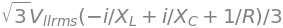
\includegraphics[width=0.7\linewidth]{files/f6dc889199220cab1097f0e3102fd714.png}

\subparagraph{Calculate Load Phase Angle}

\begin{verbatim}
angle_Y = sp.arg(Y_total)
angle_Y
\end{verbatim}


\includegraphics[width=0.7\linewidth]{files/ebf6da891e3f10797c8e02ff4e18ba92.png}

\subparagraph{Correct Phase Angle for Switch Closing at Source Current = 0A}

\begin{verbatim}
theta = pi / 2 - angle_Y
theta
\end{verbatim}


\includegraphics[width=0.7\linewidth]{files/a4af31e6964737762af331d36b1096da.png}

\subparagraph{Phase Voltage in Phasor Form}

\begin{verbatim}
V_ph_adjusted = V_ph_rms * exp(I * theta)
V_ph_adjusted
\end{verbatim}

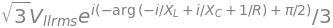
\includegraphics[width=0.7\linewidth]{files/59a0fe4e12bb9652cd276c22ff7686b4.png}

\subparagraph{Magnitude of Phase Voltage}

\begin{verbatim}
v0_sym = sqrt(2) * sp.re(V_ph_adjusted)
v0_sym
\end{verbatim}

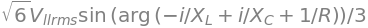
\includegraphics[width=0.7\linewidth]{files/484c2a1ca4188c1004fc9b997fb653a7.png}

\subparagraph{Calculate RMS Inductor Current}

\begin{verbatim}
I_L_rms = V_ph_adjusted / Z_L
I_L_rms
\end{verbatim}


\includegraphics[width=0.7\linewidth]{files/0146fe48534eea974acf671bde866abd.png}

\begin{verbatim}
i_L0_sym = sp.sqrt(2) * sp.re(I_L_rms)
i_L0_sym
\end{verbatim}

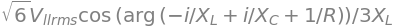
\includegraphics[width=0.7\linewidth]{files/f593180b04b8fc49006118222afb0154.png}

\begin{verbatim}
# Symbolic
display(sp.Eq(symbols(r'\angle\;Y_{total}'), angle_Y))
display(sp.Eq(symbols(r'\theta'), theta))
\end{verbatim}


\includegraphics[width=0.7\linewidth]{files/c9ed7faba1cd21b48fbc5f33f260e007.png}


\includegraphics[width=0.7\linewidth]{files/c7263651f972499a50ba6bf49749bb80.png}

\begin{verbatim}
# Numerical
subs_num = numerical_subs.copy()
subs_num
\end{verbatim}


\includegraphics[width=0.7\linewidth]{files/acfd66337a69665499ce50d439c15e78.png}

\begin{verbatim}
# Restate Xc in ohms
Xc_num
\end{verbatim}


\includegraphics[width=0.7\linewidth]{files/a1c593464ece0d5abd9ea507659f38b4.png}

\begin{verbatim}
subs_num.update({XC: Xc_num})
subs_num
\end{verbatim}


\includegraphics[width=0.7\linewidth]{files/a8bf00c7ead212786af07b37058f4e23.png}

\subparagraph{Substitute into $V_0$ and Evaluate}

\begin{verbatim}
v0_sym
\end{verbatim}

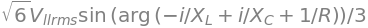
\includegraphics[width=0.7\linewidth]{files/484c2a1ca4188c1004fc9b997fb653a7.png}

\begin{verbatim}
v0_num = float(v0_sym.subs(subs_num).doit().evalf())
v0_num
\end{verbatim}


\includegraphics[width=0.7\linewidth]{files/a56df11f8ad6aa2ecdea788b8f74defd.png}

\begin{verbatim}
i_L0_num = float(i_L0_sym.subs(subs_num).doit().evalf())
i_L0_num
\end{verbatim}


\includegraphics[width=0.7\linewidth]{files/de647a1e1c91195184831efebe3f62a1.png}

\subparagraph{Phase Angle of Load Impedances $\angle Y$ in $\left[degrees\right]$:}

\begin{verbatim}
angle_Y_num = float(angle_Y.subs(subs_num).doit().evalf() * 180 / sp.pi)
angle_Y_num
\end{verbatim}


\includegraphics[width=0.7\linewidth]{files/ebbb6257536ce04864ee63d522e0a42e.png}

\subparagraph{Phase of Voltage $\theta_V$ in $\left[degrees\right]$:}

\begin{verbatim}
theta_num = float(theta.subs(subs_num).doit().evalf() * 180 / sp.pi)
theta_num
\end{verbatim}


\includegraphics[width=0.7\linewidth]{files/9f65e1b0ba6f3eff1a5c9f00dff88403.png}

\subparagraph{Total Load Current $I_{total}$ in $\left[Amps\right]$:}

\begin{verbatim}
I_total_mag = float(Abs(I_total_rms.subs(subs_num)).doit().evalf())
I_total_mag
\end{verbatim}


\includegraphics[width=0.7\linewidth]{files/3c01c7822f6f8b9aae9292441b302b25.png}

\begin{verbatim}
print(f"Numerical |I_total|_rms = {I_total_mag:.0f} A")
print(f"angle(Y_total) = {angle_Y_num:.2f} deg")
print(f"theta_V = {theta_num:.2f} deg")
print(f"v_C(0+) = {v0_num:.0f} V")
print(f"i_L(0+) = {i_L0_num:.0f} A")
\end{verbatim}

\begin{verbatim}
Numerical |I_total|_rms = 12019 A
angle(Y_total) = -33.69 deg
theta_V = 123.69 deg
v_C(0+) = -7845 V
i_L(0+) = 11767 A
\end{verbatim}

\textbf{Output (Symbolic):}

\begin{equation}
\angle Y_{total} = \arg\left(\frac{i Q_{c3ph}}{V_{llrms}^{2}} - \frac{i}{X_{L}} + \frac{1}{R}\right)
\end{equation}

\begin{equation}
\theta = - \arg\left(\frac{i Q_{c3ph}}{V_{llrms}^{2}} - \frac{i}{X_{L}} + \frac{1}{R}\right) + \frac{\pi}{2}
\end{equation}

\textbf{Numerical Values:}

$|I_{total}|_{rms} = 12019 \left[A\right]$\newline
$\angle\left(Y_{total}\right) = -33.69 \left[deg\right]$\newline
$\theta_V = 123.69 \left[deg\right]$ \newline

$v_{C}\left(0^+\right) = -7845 \left[V\right]$\newline
$i_{L}\left(0^+\right) = 11767 \left[A\right]$

\subparagraph{Step 3: Initial Conditions at $t=0^+$}

Post-switching: \newline
\begin{equation}
v_{C}\left(0^+\right) = v\left(0\right) \; (continuous)
\end{equation}

\begin{equation}
i_{L}\left(0^+\right) = i_{L}\left(0\right) \; (continuous)
\end{equation}

\begin{equation}
\frac{dv_C}{dt}\left(0^+\right) = - \frac{\left[i_{R}\left(0\right) + i_{L}\left(0\right)\right]}{C}
\end{equation}

\begin{equation}
KCL: i_C + i_R + i_L = 0
\end{equation}

\begin{verbatim}
dv0_num = ( - v0_num / 1 - i_L0_num) / C_num

print(f"v_C(0+) = {v0_num:.0f} V")
print(f"i_L(0+) = {i_L0_num:.0f} A")
print(f"dv_C/dt(0+) = {dv0_num:.2e} V/s")
\end{verbatim}

\begin{verbatim}
v_C(0+) = -7845 V
i_L(0+) = 11767 A
dv_C/dt(0+) = -4.44e+6 V/s
\end{verbatim}

\textbf{Output:} \newline

$v_{C}(0^+) = -7845 \left[V\right]$ \newline

$i_{L}(0^+) = 11767 \left[A\right]$ \newline

$\frac{dv_C}{dt}(0^+) = -4.44e+06 \left[\frac{V}{s}\right]$

\subparagraph{Step 4: Time-Domain Differential Equations}

Post-switching: Parallel RLC, voltage $v(t)$ common.

KCL:
\begin{equation}
C \frac{dv}{dt} + \frac{v}{R} + i_L = 0, \; with \frac{di_L}{dt} = \frac{v}{L}
\end{equation}

Differentiate KCL:
\begin{equation}
C \frac{d^2v}{dt^2} + \left(\frac{1}{R}\right) \frac{dv}{dt} + \left(\frac{1}{L}\right) v = 0
\end{equation}

Differential Equation:
\begin{equation}
\frac{d^2v}{dt^2} + \left(\frac{1}{R C}\right) \frac{dv}{dt} + \left(\frac{1}{L C}\right) v = 0
\end{equation}

Characteristic Equation:
\begin{equation}
s^2 + \left(\frac{1}{R C}\right) s + \left(\frac{1}{L C}\right) = 0
\end{equation}

Define:
\begin{equation}
\alpha = \frac{1}{2 R C}, \; \omega_0 = \frac{1}{\sqrt{L C}},\; \zeta = \frac{\alpha}{\omega_0} <\;1 \;(underdamped)
\end{equation}

\begin{verbatim}
t = symbols('t', real=True)

L_for_de = symbols('L', real=True, positive=True)
C_for_de = symbols('C', real=True, positive=True)
v = sp.Function('v')(t)
eq_diff_v_presub = sp.Eq(sp.diff(v, t, 2) + (1/(R*C_for_de)) * sp.diff(v, t) + (1/(L_for_de*C_for_de)) * v, 0)

display(eq_diff_v_presub)
\end{verbatim}

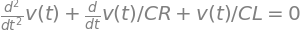
\includegraphics[width=0.7\linewidth]{files/2c197445aa21050866f60155e8e33335.png}

\begin{verbatim}
eq_diff_v = sp.Eq(sp.diff(v, t, 2) + (1/(R*C)) * sp.diff(v, t) + (1/(L*C)) * v, 0)

display(eq_diff_v)
\end{verbatim}


\includegraphics[width=0.7\linewidth]{files/326d959027842c14872363836f381c44.png}

\textbf{Output (Symbolic):}

\begin{equation}
\frac{d^{2}}{d t^{2}} v\left(t \right) + \frac{V_{llrms}^{2} \omega \frac{d}{d t} v\left(t \right)}{Q_{c3ph} R} + \frac{V_{llrms}^{2} \omega^{2} v\left(t \right)}{Q_{c3ph} X_{L}} = 0
\end{equation}

\subparagraph{Step 5: Laplace-Domain Solution}

Unilateral Laplace $(t\geq 0)$ Transform DE:
\begin{equation}
s^2 V\left(s\right) - s v\left(0\right) - v^{\prime}\left(0\right) + \frac{1}{R C} \left[s V\left(s\right) - v\left(0\right)\right] + \frac{1}{L C} V \left(s\right) = 0
\end{equation}

\begin{equation}
V\left(s\right) = \frac{\left[s v\left(0\right) + v^\prime\left(0\right)\right]}{\left[s^2 + \frac{1}{R C} s + \frac{1}{L C}\right]}
\end{equation}

For $i_{L}\left(s\right)$:
\begin{equation}
i_{L}\left(s\right) = \frac{\left[s I_{L}\left(0\right) + \frac{v(0)}{L}\right]}{\left[s² + \frac{1}{R C} s + \frac{1}{L C}\right]}
\end{equation}

\begin{verbatim}
s = symbols('s')
I_L0 = symbols('I_{L0}')
V0 = symbols('V_0')
V_s = sp.Function('V')(s)
denom = s**2 + (1/(R*C_for_de))*s + 1/(L_for_de*C_for_de)
dv0_sym = ( -V0 / R - I_L0) / C_for_de  # From Step 3 symbolic
V_s_sol_for_de = (s * V0 + dv0_sym) / denom

display(sp.Eq(V_s, V_s_sol_for_de))
\end{verbatim}

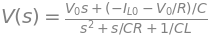
\includegraphics[width=0.7\linewidth]{files/7cc99fd51484b6a2ec2aee09d00a0f4b.png}

\begin{verbatim}
V_s = sp.Function('V')(s)
denom = s**2 + (1/(R*C))*s + 1/(L*C)
dv0_sym = ( -V0 / R - I_L0) / C  # From Step 3 symbolic
V_s_sol = (s * V0 + dv0_sym) / denom

display(sp.Eq(V_s, V_s_sol))
\end{verbatim}

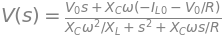
\includegraphics[width=0.7\linewidth]{files/a51c1d39c9de13ff23afd8ca154b2479.png}

\textbf{Output (Symbolic):}

\begin{equation}
V\left(s \right) = \frac{V_{0} s + \frac{V_{llrms}^{2} \omega \left(- I_{L0} - \frac{V_{0}}{R}\right)}{Q_{c3ph}}}{s^{2} + \frac{V_{llrms}^{2} \omega s}{Q_{c3ph} R} + \frac{V_{llrms}^{2} \omega^{2}}{Q_{c3ph} X_{L}}}
\end{equation}

Simplified:
\begin{equation}
V\left(s\right) = \frac{\left[s V_0 + v^\prime\left(0\right)\right]}{\left[s^2 + \frac{1}{R C} s + {\omega_0}^2\right]}
\end{equation}

\subparagraph{Step 6: Inverse Laplace Transform (Time-Domain Responses)}

Underdamped:
\begin{equation}
v(t) = e^{-\alpha t} [A\;cos(\omega_d t) + B\;sin(\omega_d t)]
\end{equation}

\begin{equation}
A = V_0
\end{equation}

\begin{equation}
B = \frac{\left[v^{\prime}\left(0\right) + \alpha V_0\right]}{\omega_d}
\end{equation}

\begin{equation}
i_L\left(t\right) = e^{-\alpha t} [D\;cos(\omega_d t) + E\;sin(\omega_d t)]
\end{equation}

\begin{equation}
D = I_{L0}
\end{equation}

\begin{equation}
E = \frac{\left[\frac{V_0}{L} + \alpha I_{L0}\right]}{\omega_d}
\end{equation}

\begin{verbatim}
alpha = 1 / (2 * R * C)
alpha
\end{verbatim}


\includegraphics[width=0.7\linewidth]{files/1450cc16028156de08abefe681c10c08.png}

\begin{verbatim}
omega0 = 1 / sqrt(L * C)
omega0
\end{verbatim}


\includegraphics[width=0.7\linewidth]{files/5bd638c3abbe755092e495c897367985.png}

\begin{verbatim}
omegad = sqrt(omega0**2 - alpha**2)
omegad
\end{verbatim}

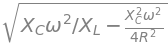
\includegraphics[width=0.7\linewidth]{files/e530c9f11ff7a3636aa2a1d86eb4b24a.png}

\begin{verbatim}
zeta = alpha / omega0
zeta
\end{verbatim}


\includegraphics[width=0.7\linewidth]{files/a580019b23257be411a8a9b499247ee5.png}

\begin{verbatim}
A = V0
A
\end{verbatim}


\includegraphics[width=0.7\linewidth]{files/da411f5a067e2e707e90b6350a9ad5f7.png}

\begin{verbatim}
B = (dv0_sym + alpha * V0) / omegad
B
\end{verbatim}

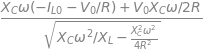
\includegraphics[width=0.7\linewidth]{files/614708ee1168d7b579f937cbbb5a8d4b.png}

\begin{verbatim}
v_standard = exp( -alpha * t) * (A * cos(omegad * t) + B * sin(omegad * t))
v_standard
\end{verbatim}

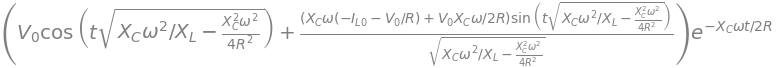
\includegraphics[width=0.7\linewidth]{files/be724ecf6b8f6f0840a8bcfac54c50d3.png}

\begin{verbatim}
D = I_L0
D
\end{verbatim}


\includegraphics[width=0.7\linewidth]{files/ca0b92a73b4f0db6452dde754af4f23f.png}

\begin{verbatim}
E = (V0 / L + alpha * I_L0) / omegad
E
\end{verbatim}

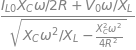
\includegraphics[width=0.7\linewidth]{files/e433bacc72961813ee6ba9fd2dd88d09.png}

\begin{verbatim}
i_L_standard = exp( -alpha * t) * (D * cos(omegad * t) + E * sin(omegad * t))
i_L_standard
\end{verbatim}

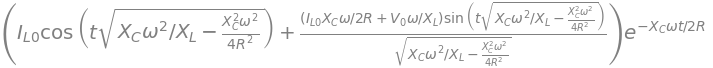
\includegraphics[width=0.7\linewidth]{files/8f2881a72c4c9b3e0ede94e15952bb69.png}

\subparagraph{Show Symbolic Equations}

\begin{verbatim}
display(sp.Eq(sp.Function('v')(t), v_standard))
\end{verbatim}

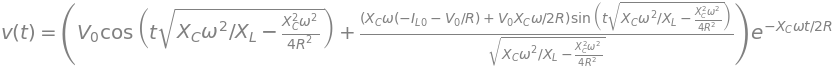
\includegraphics[width=0.7\linewidth]{files/dd1837dd515772a2017730246a9b1d62.png}

\begin{verbatim}
display(sp.Eq(sp.Function('i_L')(t), i_L_standard))
\end{verbatim}

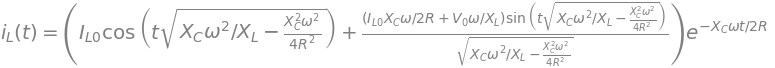
\includegraphics[width=0.7\linewidth]{files/9ec46cd9f90526f68a12ce82f34306d6.png}

\subparagraph{Evaluate Numerically}

\begin{verbatim}
subs_num_full = numerical_subs.copy()
subs_num_full
\end{verbatim}


\includegraphics[width=0.7\linewidth]{files/acfd66337a69665499ce50d439c15e78.png}

\begin{verbatim}
subs_num_full.update({R:1, XL:1, XC:Xc_num, V0:v0_num, I_L0:i_L0_num, C:C_num, L:L_num})
subs_num_full
\end{verbatim}


\includegraphics[width=0.7\linewidth]{files/051d343599e249cc27057084a6609191.png}

\begin{verbatim}
alpha_num = float(alpha.subs(subs_num_full).doit().evalf())
alpha_num
\end{verbatim}


\includegraphics[width=0.7\linewidth]{files/9f76e209b7352f26925c633239bd1dd2.png}

\begin{verbatim}
omega0_num = float(omega0.subs(subs_num_full).doit().evalf())
omega0_num
\end{verbatim}


\includegraphics[width=0.7\linewidth]{files/44fe3a867d8b597a9f8d1187b552d25c.png}

\begin{verbatim}
omegad_num = float(omegad.subs(subs_num_full).doit().evalf())
omegad_num
\end{verbatim}


\includegraphics[width=0.7\linewidth]{files/df78030e3dabc2a4faeccd6155a40d89.png}

\begin{verbatim}
zeta_num = float(zeta.subs(subs_num_full).doit().evalf())
zeta_num
\end{verbatim}


\includegraphics[width=0.7\linewidth]{files/7e7f598bfc5e52ae984029e342c13ea1.png}

\begin{verbatim}
A_num = v0_num
A_num
\end{verbatim}


\includegraphics[width=0.7\linewidth]{files/a56df11f8ad6aa2ecdea788b8f74defd.png}

\begin{verbatim}
B_num = (dv0_num + alpha_num * v0_num) / omegad_num
B_num
\end{verbatim}


\includegraphics[width=0.7\linewidth]{files/82112d9e870d3e57e2ebbabd06c2ed1d.png}

\begin{verbatim}
D_num = i_L0_num
D_num
\end{verbatim}


\includegraphics[width=0.7\linewidth]{files/de647a1e1c91195184831efebe3f62a1.png}

\begin{verbatim}
E_num = (v0_num / L_num + alpha_num * i_L0_num) / omegad_num
E_num
\end{verbatim}


\includegraphics[width=0.7\linewidth]{files/327547e657c00ad4ab9430b4c75238bb.png}

\begin{verbatim}
print(f'$5$')
\end{verbatim}

\begin{verbatim}
$5$
\end{verbatim}

\begin{verbatim}
print(f"alpha = {alpha_num:.1f} [rad/s]")
print(f"omega_0 = {omega0_num:.1f} [rad/s]")
print(f"zeta = {zeta_num:.3f}")
print(f"omega_d = {omegad_num:.1f} [rad/s]")
print(f"A = {A_num:.0f} [V], B = {B_num:.0f} [V]")
print(f"D = {D_num:.0f} [A], E = {E_num:.0f} [A]")
\end{verbatim}

\begin{verbatim}
alpha = 565.5 [rad/s]
omega_0 = 653.0 [rad/s]
zeta = 0.866
omega_d = 326.5 [rad/s]
A = -7845 [V], B = -27175 [V]
D = 11767 [A], E = 11323 [A]
\end{verbatim}

\textbf{Output (Symbolic):}

\begin{equation}
v\left(t \right) = \left(V_{0} \cos\left(t \sqrt{\frac{V_{llrms}^{2} \omega^{2}}{Q_{c3ph} X_{L}} - \frac{V_{llrms}^{4} \omega^{2}}{4 Q_{c3ph}^{2} R^{2}}}\right) + \frac{\left(\frac{V_{llrms}^{2} \omega \left(- I_{L0} - \frac{V_{0}}{R}\right)}{Q_{c3ph}} + \frac{V_{0} V_{llrms}^{2} \omega}{2 Q_{c3ph} R}\right) \sin\left(t \sqrt{\frac{V_{llrms}^{2} \omega^{2}}{Q_{c3ph} X_{L}} - \frac{V_{llrms}^{4} \omega^{2}}{4 Q_{c3ph}^{2} R^{2}}}\right)}{\sqrt{\frac{V_{llrms}^{2} \omega^{2}}{Q_{c3ph} X_{L}} - \frac{V_{llrms}^{4} \omega^{2}}{4 Q_{c3ph}^{2} R^{2}}}}\right) e^{- \frac{V_{llrms}^{2} \omega t}{2 Q_{c3ph} R}}
\end{equation}

\begin{equation}
i_{L}\left(t \right) = \left(I_{L0} \cos\left(t \sqrt{\frac{V_{llrms}^{2} \omega^{2}}{Q_{c3ph} X_{L}} - \frac{V_{llrms}^{4} \omega^{2}}{4 Q_{c3ph}^{2} R^{2}}}\right) + \frac{\left(\frac{I_{L0} V_{llrms}^{2} \omega}{2 Q_{c3ph} R} + \frac{V_{0} \omega}{X_{L}}\right) \sin\left(t \sqrt{\frac{V_{llrms}^{2} \omega^{2}}{Q_{c3ph} X_{L}} - \frac{V_{llrms}^{4} \omega^{2}}{4 Q_{c3ph}^{2} R^{2}}}\right)}{\sqrt{\frac{V_{llrms}^{2} \omega^{2}}{Q_{c3ph} X_{L}} - \frac{V_{llrms}^{4} \omega^{2}}{4 Q_{c3ph}^{2} R^{2}}}}\right) e^{- \frac{V_{llrms}^{2} \omega t}{2 Q_{c3ph} R}}
\end{equation}

\textbf{Numerical:} \newline

$\alpha$ = $565.5\;\left[\frac{rad}{s}\right]$ \newline

$\omega_0$ = $653.0\;\left[\frac{rad}{s}\right]$ \newline

$\omega_d$ = $326.5\;\left[\frac{rad}{s}\right]$ \newline

$\zeta$ = 0.866

$A$ = -7845 $\left[V\right]$, B = -27175 $\left[V\right]$\newline
$D$ = 11767 $\left[A\right]$, E = 11323 $\left[A\right]$

\subparagraph{Step 7: Numerical Simulation and Plots}

Lambdify for evaluation. t=0 to 0.1 s, dt=1 $\mu$s. Verify ICs via eval at t=0.

\begin{verbatim}
v_func = lambda tt: np.exp( -alpha_num * tt) * (A_num * np.cos(omegad_num * tt) + B_num * np.sin(omegad_num * tt))
v_func
\end{verbatim}

\begin{verbatim}
<function __main__.<lambda>(tt)>
\end{verbatim}

\begin{verbatim}
i_L_func = lambda tt: np.exp( -alpha_num * tt) * (D_num * np.cos(omegad_num * tt) + E_num * np.sin(omegad_num * tt))
i_L_func
\end{verbatim}

\begin{verbatim}
<function __main__.<lambda>(tt)>
\end{verbatim}

\begin{verbatim}
t_num = np.arange(0, 0.04, 1e -4)
\end{verbatim}

\begin{verbatim}
v_plot = v_func(t_num)
\end{verbatim}

\begin{verbatim}
i_L_plot = i_L_func(t_num)
\end{verbatim}

\subparagraph{Verify Results}

\begin{verbatim}
print(f"v_C(0) = {v_plot[0]:.0f} V (should be {v0_num:.0f} V)")
\end{verbatim}

\begin{verbatim}
v_C(0) = -7845 V (should be -7845 V)
\end{verbatim}

\begin{verbatim}
print(f"i_L(0) = {i_L_plot[0]:.0f} A (should be {i_L0_num:.0f} A)")
\end{verbatim}

\begin{verbatim}
i_L(0) = 11767 A (should be 11767 A)
\end{verbatim}

\begin{verbatim}
dv_plot_0 = np.gradient(v_plot, t_num)[0]
print(f"dv_C/dt(0) \approx {dv_plot_0:.2e} V/s (should be {dv0_num:.2e} V/s)")
\end{verbatim}

\begin{verbatim}
dv_C/dt(0) \approx -4.03e+06 V/s (should be -4.44e+6 V/s)
\end{verbatim}

\begin{verbatim}
# Numerical Simulation and Plots

# Extended plots: Steady -state pre -switching (t < 0) and transients post -switching (t >= 0).
# Time: -0.1 to 0.1 s (few cycles before/after), dt=1 \mus.
# Steady -state:
# - Source voltage v_s(t) = sqrt(2) V_ph_rms cos( \omega t + \theta)
# - Source current i_total(t) = sqrt(2) |I_total| cos( \omega t + \theta + ∠Y_total)
# - Steady -state v_C(t) = v_s(t) (parallel, directly across source)
# - Steady -state i_L(t) = sqrt(2) |I_L_rms| cos( \omega t + \theta + ∠I_L)
# Annotate t=0 with vertical line "Switch Opens".

# Lambdify transients (post t=0)
v_trans_func = lambda tt: np.exp( -alpha_num * tt) * (A_num * np.cos(omegad_num * tt) + B_num * np.sin(omegad_num * tt))
i_L_trans_func = lambda tt: np.exp( -alpha_num * tt) * (D_num * np.cos(omegad_num * tt) + E_num * np.sin(omegad_num * tt))
\end{verbatim}

\begin{verbatim}
# Time vector: -0.1 to 0.1 s
t_num = np.arange( -0.1, 0.1, 1e -4)
switch_time = 0  # t=0
\end{verbatim}

\begin{verbatim}
# Steady -state functions (for t < 0)
V_ph_peak = np.sqrt(2) * 10000
V_ph_peak
\end{verbatim}


\includegraphics[width=0.7\linewidth]{files/232333ad4a766ae88ef5e5b47d1bc04a.png}

\begin{verbatim}
I_total_peak = np.sqrt(2) * I_total_mag
I_total_peak
\end{verbatim}


\includegraphics[width=0.7\linewidth]{files/ac288b1477c17fe1537f19592ab48d47.png}

\begin{verbatim}
I_L_peak = np.sqrt(2) * i_L0_num
I_L_peak
\end{verbatim}


\includegraphics[width=0.7\linewidth]{files/2a23a8c30c3dbc2a2ac4c25d9d46bf55.png}

\begin{verbatim}
angle_I_L = float(arg(I_L_rms.subs(subs_num)).doit().evalf() * 180 / pi)
print("Computed angle_I_L = {:.2f} deg".format(angle_I_L))
\end{verbatim}

\begin{verbatim}
Computed angle_I_L = 33.69 deg
\end{verbatim}

\begin{verbatim}
# Numerical omega
omega_num = 377.0

v_s_ss = lambda tt: V_ph_peak * np.cos(omega_num * tt + theta_num * np.pi / 180)
i_total_ss = lambda tt: I_total_peak * np.cos(omega_num * tt + theta_num * np.pi / 180 + angle_Y_num * np.pi / 180)
v_C_ss = v_s_ss  # Same as source
i_L_ss = lambda tt: I_L_peak * np.cos(omega_num * tt + theta_num * np.pi / 180 + angle_I_L * np.pi / 180)

# Combined waveforms
v_C_combined = np.where(t_num < switch_time, v_C_ss(t_num), v_trans_func(t_num))
i_L_combined = np.where(t_num < switch_time, i_L_ss(t_num), i_L_trans_func(t_num))

# Verify ICs (continuity at t=0)
idx_switch = np.argmin(np.abs(t_num - switch_time))
print(f"v_C( -) \approx {v_C_ss(t_num[idx_switch -1]):.0f} V, v_C(0+) = {v_trans_func(t_num[idx_switch]):.0f} V")
print(f"i_L( -) \approx {i_L_ss(t_num[idx_switch -1]):.0f} A, i_L(0+) = {i_L_trans_func(t_num[idx_switch]):.0f} A")
dv_plot_0 = np.gradient(v_C_combined, t_num)[idx_switch]
print(f"dv_C/dt(0) \approx {dv_plot_0:.2e} V/s (should be {dv0_num:.2e})")

# Plots: 2 figures - one for voltages (source/v_C), one for currents (source/i_total, i_L)
fig1, (ax1a, ax1b) = plt.subplots(2, 1, figsize=(12, 10))
# Source voltage and v_C
ax1a.plot(t_num * 1000, v_s_ss(t_num) / 1000, 'b - -', linewidth=1.5, label='Source Voltage v_s(t)')
ax1a.plot(t_num * 1000, v_C_combined / 1000, 'r -', linewidth=1.5, label='Capacitor Voltage v_C(t)')
ax1a.axvline(x=switch_time * 1000, color='k', linestyle=':', linewidth=2, label='Switch Opens')
ax1a.annotate('Switch Opens\n(i_total=0)', xy=(0, v0_num / 1000), xytext=(5, v0_num / 1000 + 2),
              arrowprops=dict(arrowstyle=' ->', color='black'), fontsize=10)
ax1a.grid(True)
ax1a.set_xlabel('Time (ms)')
ax1a.set_ylabel('Voltage (kV)')
ax1a.set_title('Source Voltage and Capacitor Voltage (Steady -State + Transient)')
ax1a.set_xlim([ -100, 100])
ax1a.legend()

# Source current and i_L (steady -state only for i_total, as post -switch no source current)
ax1b.plot(t_num * 1000, i_total_ss(t_num) / 1000, 'g - -', linewidth=1.5, label='Source Current i_total(t)')
ax1b.plot(t_num * 1000, i_L_combined / 1000, 'm -', linewidth=1.5, label='Inductor Current i_L(t)')
ax1b.axvline(x=switch_time * 1000, color='k', linestyle=':', linewidth=2)
ax1b.annotate('Switch Opens', xy=(0, i_L0_num / 1000), xytext=(5, i_L0_num / 1000 + 1),
              arrowprops=dict(arrowstyle=' ->', color='black'), fontsize=10)
ax1b.grid(True)
ax1b.set_xlabel('Time (ms)')
ax1b.set_ylabel('Current (kA)')
ax1b.set_title('Source Current and Inductor Current (Steady -State + Transient)')
ax1b.set_xlim([ -100, 100])
ax1b.legend()

plt.tight_layout()
plt.show()

# Additional plot: Zoom on transients post -switch (t=0 to 0.1 s)
fig2, (ax2a, ax2b) = plt.subplots(2, 1, figsize=(12, 10))
ax2a.plot(t_num[t_num >= 0] * 1000, v_C_combined[t_num >= 0] / 1000, 'r -', linewidth=1.5)
ax2a.grid(True)
ax2a.set_xlabel('Time (ms)')
ax2a.set_ylabel('v_C (kV)')
ax2a.set_title('Capacitor Voltage Transient (Post -Switch)')
ax2a.set_xlim([0, 100])

ax2b.plot(t_num[t_num >= 0] * 1000, i_L_combined[t_num >= 0] / 1000, 'm -', linewidth=1.5)
ax2b.grid(True)
ax2b.set_xlabel('Time (ms)')
ax2b.set_ylabel('i_L (kA)')
ax2b.set_title('Inductor Current Transient (Post -Switch)')
ax2b.set_xlim([0, 100])

plt.tight_layout()
plt.show()
\end{verbatim}

\begin{verbatim}
v_C( -) \approx -7396 V, v_C(0+) = -7845 V
i_L( -) \approx -15109 A, i_L(0+) = 11767 A
dv_C/dt(0) \approx -4.26e+06 V/s (should be -4.44e+6)
\end{verbatim}

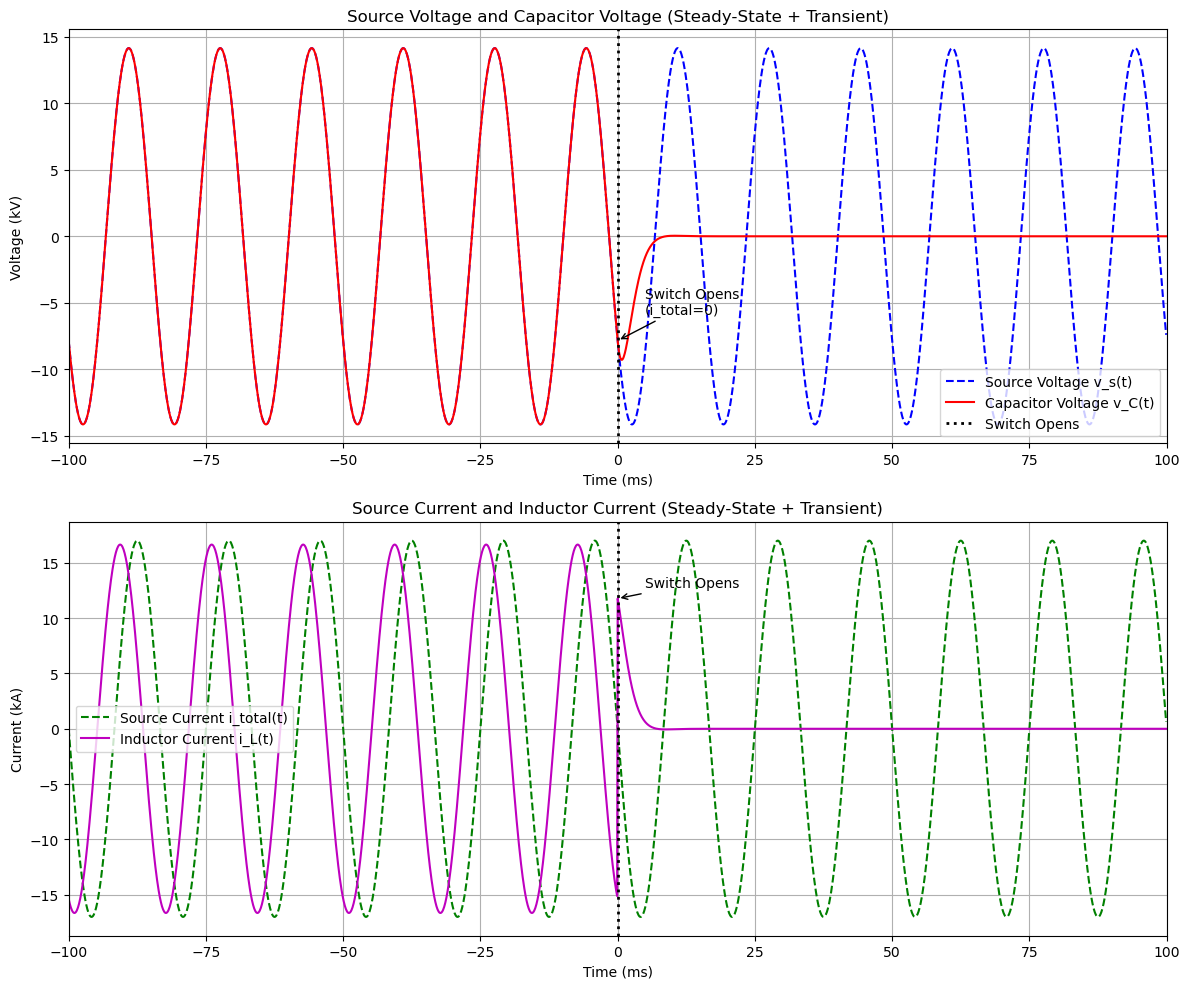
\includegraphics[width=0.7\linewidth]{files/d34f4bf0c8ca6c7ffd0705dd08ea0b46.png}

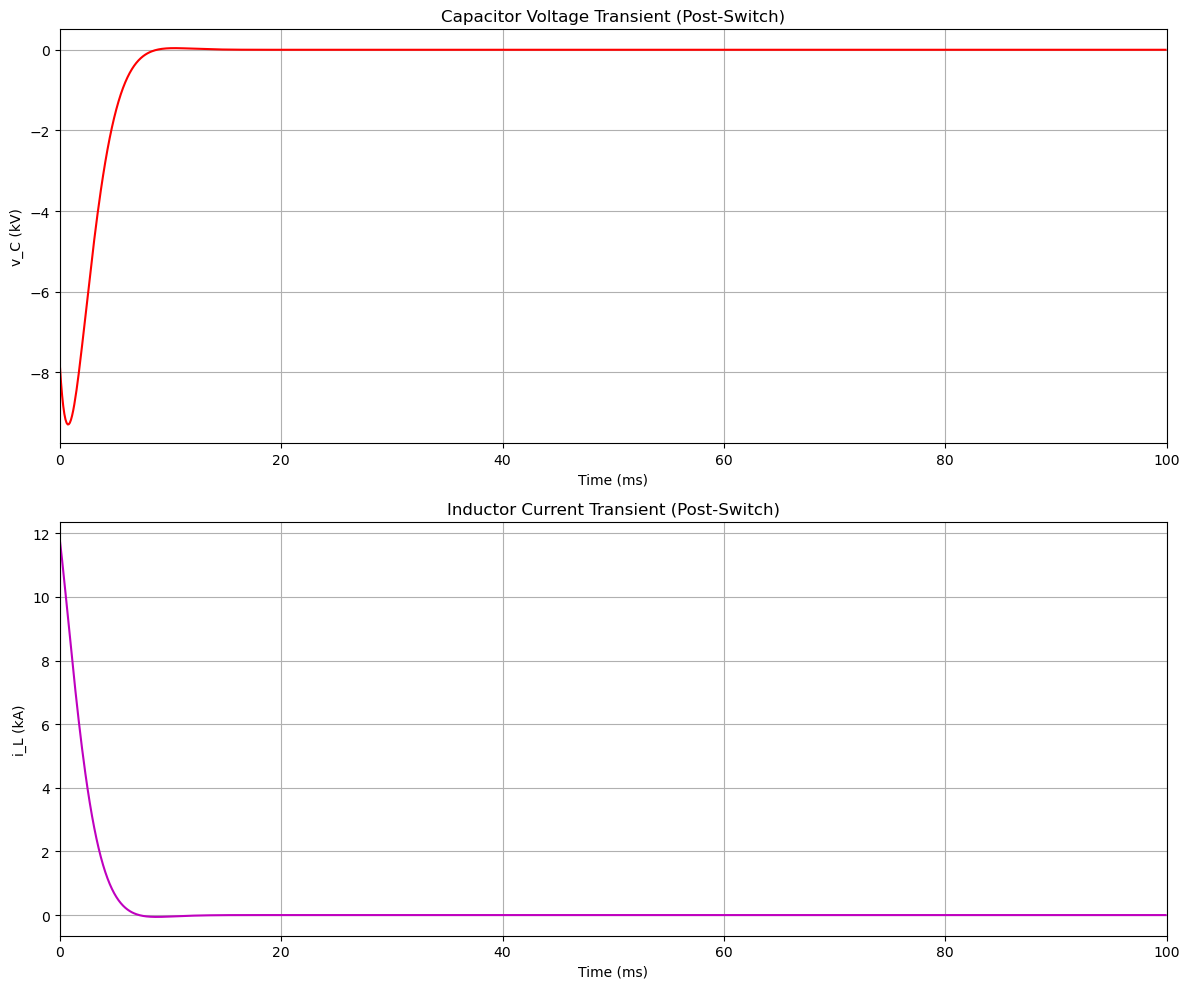
\includegraphics[width=0.7\linewidth]{files/f5fc454833afaabdcd618f0f7e233324.png}

\subparagraph{Compare to Simulation}

\begin{figure}[!htbp]
\centering
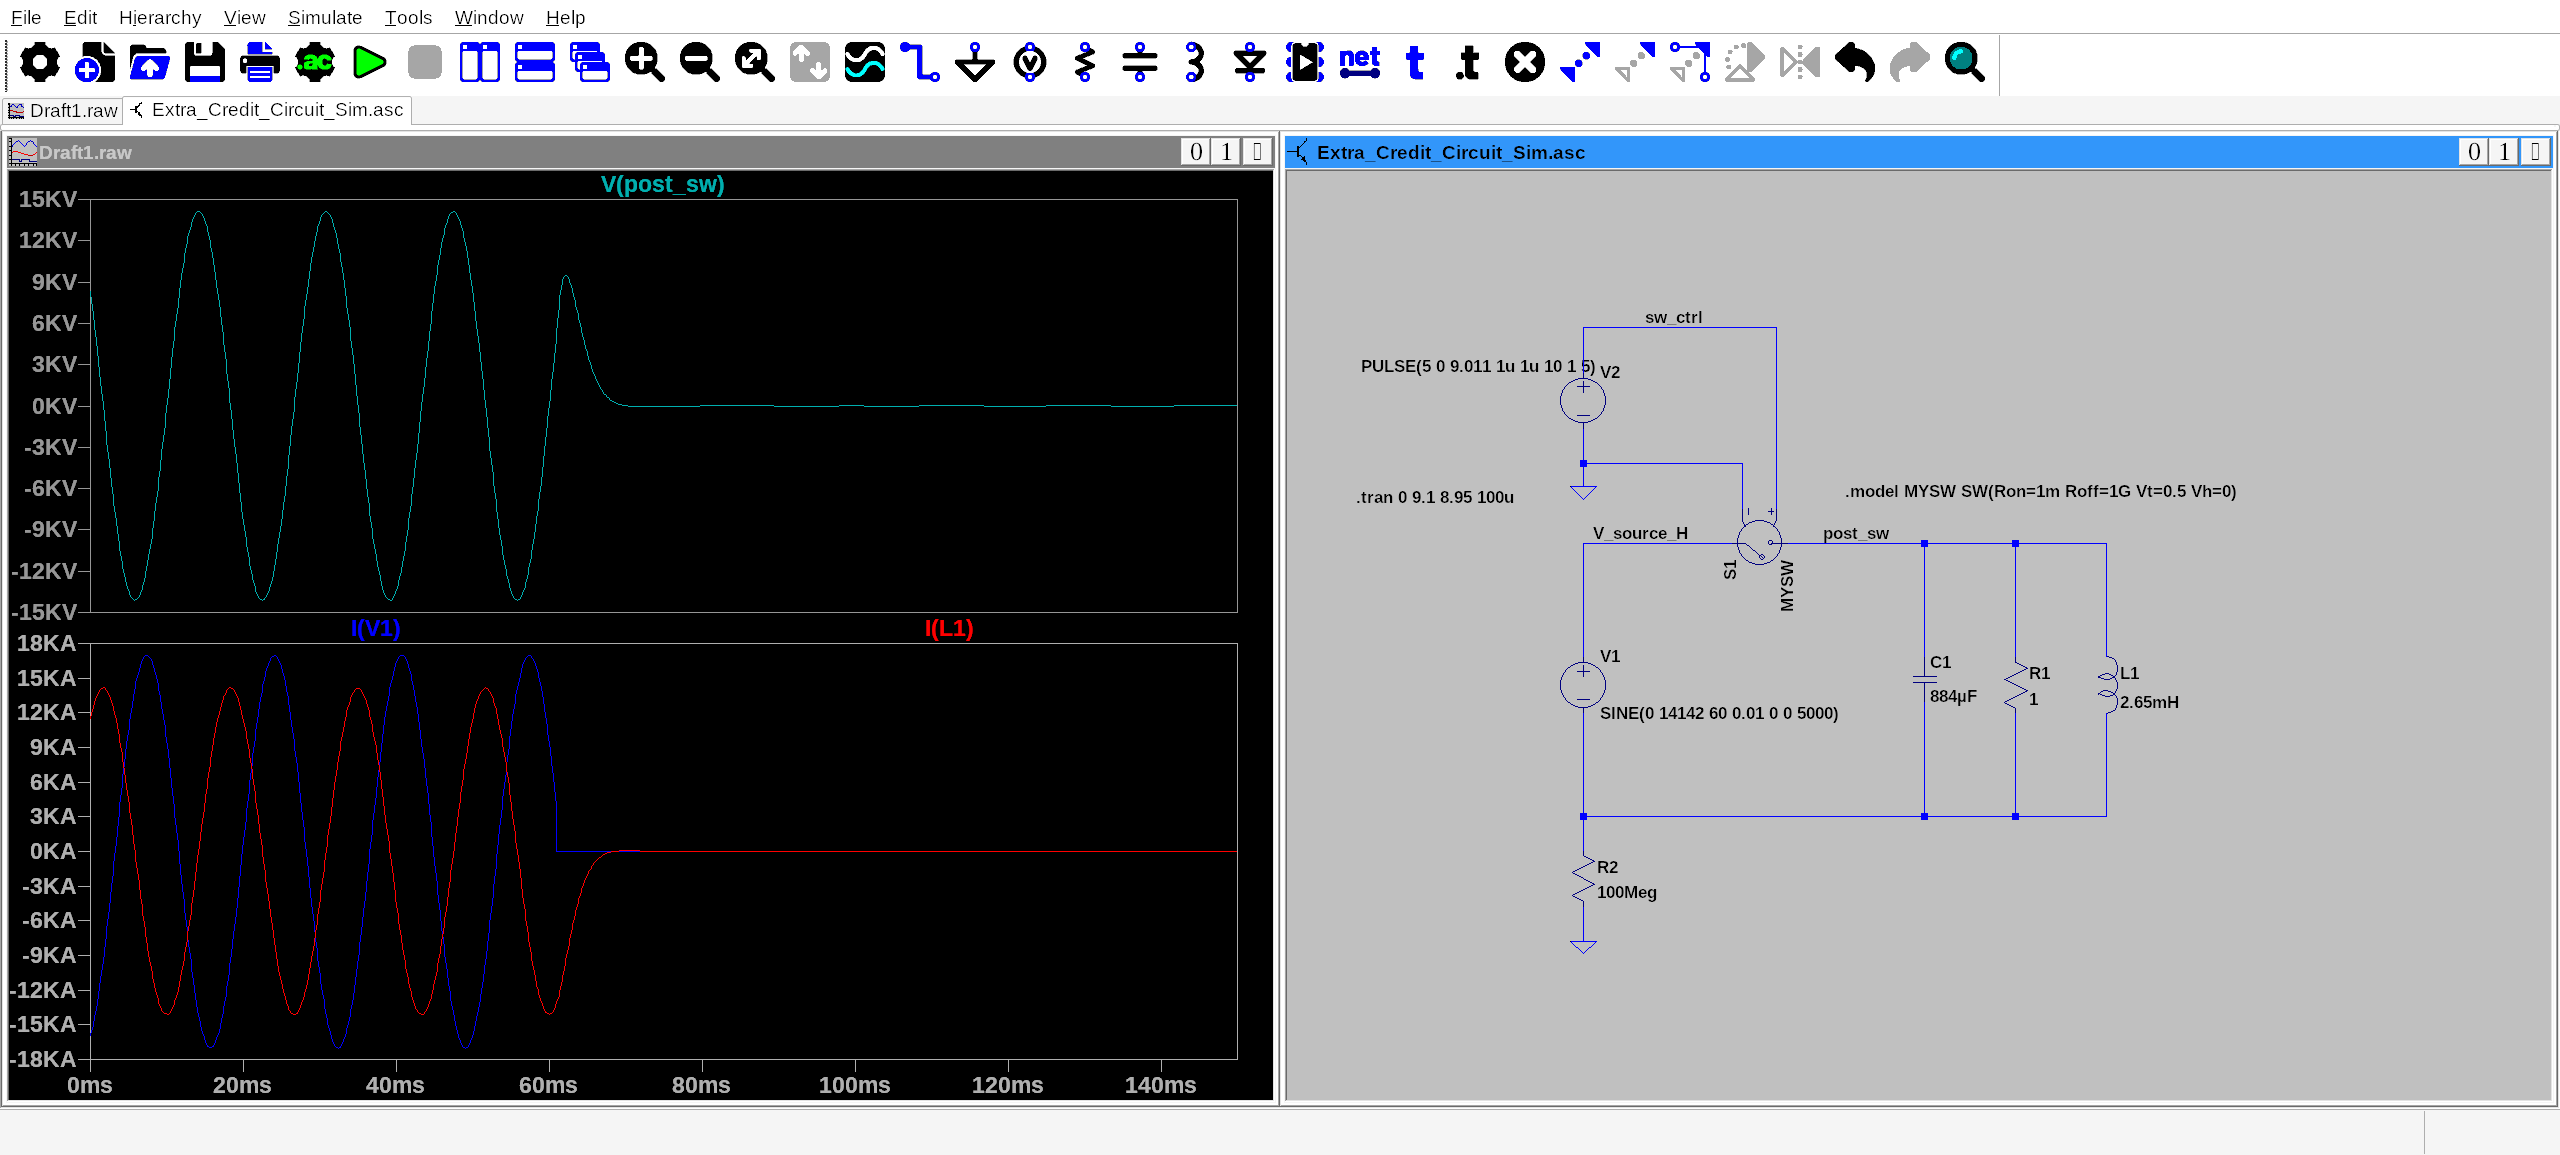
\includegraphics[width=0.7\linewidth]{files/Extra_Credit_Circuit-5034fb1c809bb7946dc6ecc1e443638f.png}
\caption[]{EEE571 Extra Credit Problem Circuit Simulation}
\label{EEE571_Extra_Credit_Fig_1}
\end{figure}